\begin{center}
\Huge
Intro til potensfunktioner
\end{center}

\section*{Potensfunktioner}
\stepcounter{section}



Vi har set på lineære funktioner, der er funktioner på formen
\begin{align*}
	f(x) = ax + b
\end{align*}
og eksponentialfunktioner, der er funktioner på formen
\begin{align*}
	g(x) = b\cdot a^x.
\end{align*}
Den næste klasse af funktioner, vi skal arbejde med er \textit{potensfunktioner}.
\begin{defn}[Potensfunktion]
	Lad $b > 0$. En funktion $f$ på formen
	\begin{align*}
		f(x) = b\cdot x^a
	\end{align*}
	kaldes for en \textit{potensfunktion.}
\end{defn}


\begin{exa}
	Funktionen $f$ givet ved
	\begin{align*}
		f(x) = 1.5 \cdot x^3
	\end{align*}
	samt funktionen $g$ givet ved
	\begin{align*}
		g(x) = 10\cdot x^{-2}
	\end{align*}
	er potensfunktioner. For $f$ er $b = 1.5$ og $a = 3$. Tilsvarende for $g$ er $b = 10$ og $a = -2$.
	Grafen for disse funktioner kan ses af Figur \ref{fig:potensgraf}.
	
	\begin{figure}[H]
		\centering
		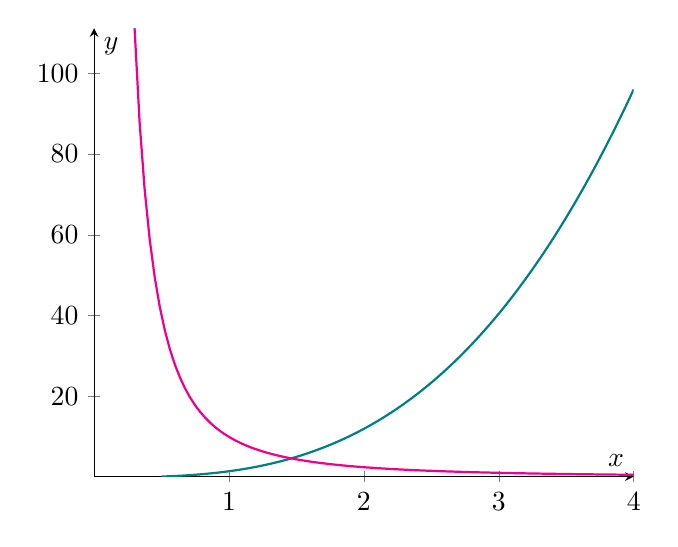
\begin{tikzpicture}
			\begin{axis}[
			axis lines = middle, 
			xmin = 0, xmax = 4,
			xlabel = $x$,
			ylabel = $y$
			]
				\addplot[color = teal, thick, domain = 0.5:4, samples = 100] {1.5*x^3};
				\addplot[color = magenta, thick, domain = 0.3:4, samples = 100] {10*x^(-2)};
			\end{axis}
		\end{tikzpicture}
		\caption{Grafer for potensfunktionerne $f$ og $g$.}
		\label{fig:potensgraf}
	\end{figure}
\end{exa}

\begin{exa}
	Vi betragter rektanglet på Figur \ref{fig:rektangel}.
	\begin{figure}[H]
		\centering
		\begin{tikzpicture}
			\draw[color = teal, thick] (-3,0) -- (3,0);
			\draw[color = teal, thick] (-3,0) -- (-3,-3);
			\draw[color = teal, thick] (-3,-3) -- (3,-3);
			\draw[color = teal, thick] (3,-3) -- (3,0);
			\draw[decorate,	decoration = {calligraphic brace, mirror, raise = 3pt, amplitude = 5pt}, thick, pen colour = {teal}] (-3,-3) --  (3,-3);
			\draw[decorate,	decoration = {calligraphic brace, raise = 3pt, amplitude = 5pt}, thick, pen colour = {teal}] (3,0) --  (3,-3);
			\node[color = teal] at (3.6,-1.5) {$x$};
			\node[color = teal] at (0,-3.6) {$2x$};
		\end{tikzpicture}
		\caption{Rektangel med højde $x$ og bredde $2x$.}
		\label{fig:rektangel}
	\end{figure}
	Dette rektangel har bredde $2x$ og højde $x$. Derfor er arealet $A$ af rektanglet givet ved
	\begin{align*}
		A(x) = 2x\cdot x = 2x^2,
	\end{align*}
	som er en potensfunktion.
\end{exa}


\subsection*{Opgave 1}

Afgør om følgende funktioner er lineære, eksponential- eller potensfunktioner. 
\begin{align*}
	&a) \ 2\cdot 3^x  &&b) \ 5\cdot x^{1.7}  \\
	&c) \ \sqrt{3}\cdot x + 9 &&d) \ 2.9\cdot e^x  \\
	&e) \ 6\cdot x^{-1} &&f) \ 200x^2  \\
	&g) \ -10x + 13 &&h) \ 2^x \\
	&i) \ x^2  &&j) \ 7+ 9x  \\
\end{align*}

\subsection*{Opgave 2}

Aflæs $a$ og $b$ for følgende potensfunktioner
\begin{align*}
	&a) \ 2\cdot x^2  &&b) \ 5\cdot x^{10} \\
	&c) \ \sqrt{3}\cdot x^{3.2} &&d) \ x^{-0.5}  \\
\end{align*}

\subsection*{Opgave 3}
På Figur \ref{fig:opgavegrafer} kan graferne for de to potensfunktioner $f$ og $g$ ses. 
\begin{figure}[H]
	\center
	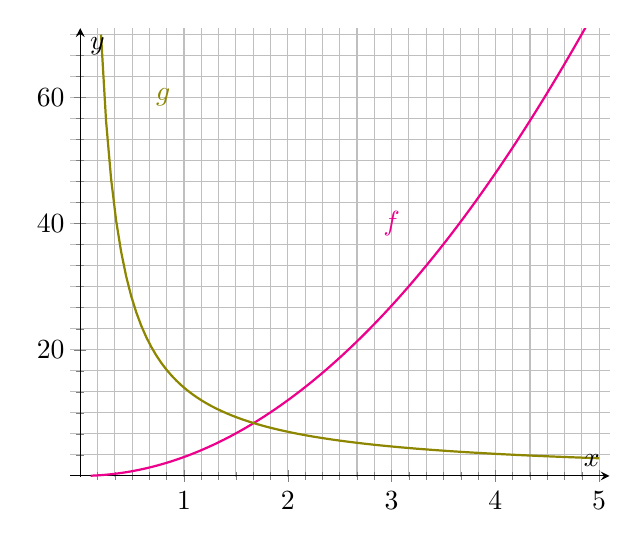
\begin{tikzpicture}
		\begin{axis}[
		axis lines = middle, 
		xmin = -0.1, xmax = 5.1,
		ymin = -0.1, ymax = 71,
		xlabel = $x$, ylabel = $y$, 
		grid = both, minor tick num = 5]
			\addplot[color = magenta, thick, domain = 0.1:5, samples = 100] {3*x^2};		
			\addplot[color = olive, thick, domain = 0.2:5, samples = 100] {14*x^(-1)};
			\node[color = olive] at (axis cs: 0.8,60) {$g$};
			\node[color = magenta] at (axis cs: 3,40) {$f$};
		\end{axis}
	\end{tikzpicture}
	\caption{Grafer for to potensfunktioner $f$ og $g$.}
	\label{fig:opgavegrafer}
\end{figure}
Brug Figur \ref{fig:opgavegrafer} til at løse følgende opgaver.
\begin{enumerate}[label=\roman*)]
	\item Bestem $f(2)$.
	\item Bestem $g(4)$.
	\item Løs ligningen $g(x) = 44$.
	\item Løs ligningen $f(x) = 30$.
	\item Løs ligningen $f(x) = g(x)$.
\end{enumerate}

\subsection*{Opgave 4}
Et rektangel har højde $4x$ og bredde $3x$. 
\begin{enumerate}[label=\roman*)]
	\item Opskriv et udtryk for arealet $A(x)$ som funktion af højden og bredden. 
	\item Bestem $a$ og $b$ i forskriften for $A$. 
	\item Bestem $A(4)$.
	\item Brug $A(x)$ til at bestemme højden og bredden af rektanglet, hvis det skal have et areal på 1200.
\end{enumerate}

\subsection*{Opgave 5}
En potensfunktion er givet ved 
\begin{align*}
	f(x) = b\cdot x^2.
\end{align*}

\begin{enumerate}[label = \roman*)]
	\item Udnyt, at $f(2) = 20$ for at bestemme $b$. 
	\item Bestem $f(4)$.
	\item Løs ligningen $f(x) = 45$.
\end{enumerate}

\subsection*{Opgave 6}
To potensfunktioner $f$ og $g$ er givet ved
\begin{align*}
	f(x) = 2 \cdot x^{2}
\end{align*}
og 
\begin{align*}
	g(x) = 1 \cdot x^{a}.
\end{align*}

\begin{enumerate}[label=\roman*)]
	\item Det oplyses, at $2\cdot f(4) = g(4)$. Brug dette til at bestemme tallet $a$.  
\end{enumerate}



\subsection*{Opgave 7 (Med Maple)}
To potensfunktioner $f$ og $g$ er givet ved
\begin{align*}
	f(x) = 2\cdot x^{0.5}
\end{align*}
og 
\begin{align*}
	g(x) = 10 \cdot x^{1.4}
\end{align*}

\begin{enumerate}[label=\roman*)]
	\item Bestem $g(3)$.
	\item Tegn graferne for $f$ og $g$ i samme koordinatsystem.
	\item Bestem skæringspunktet mellem $f$ og $g$ ved at løse en ligning. 
\end{enumerate}




\subsection*{Opgave 8 (Med Maple)}
\begin{enumerate}[label=\roman*)]
\item En cylinder har samme diameter som højde. Bestem den potensfunktion, der beskriver rumfanget af cylinderen som funktion af cylinderens radius. 
\item En kasse har bredde, højde og længde $x$. Bestem rumfanget af $x$, og afgør, hvad $a$ og $b$ er i denne potensfunktion.
\item For et bestemt objekt kan vindmodstanden på objektet beskrives ved 
\begin{align*}
F(v)= \frac{1}{2}v^2,
\end{align*}
hvor $v$ er hastigheden i $m/s$, objektet bevæger sig med, og $F$ er vindmodstanden målt i $N$. Hvad er vindmodstanden, når objektet bevæger sig med 50$m/s$? Hvor hurtigt skal objektet bevæge sig, for at modstanden på objektet er 20$N$?

\end{enumerate}

\subsection*{Opgave 9}

Vi betragter potensfunktionen $f$ givet ved
\begin{align*}
	f(x) = b\cdot x^a.
\end{align*}

\begin{enumerate}[label = \roman*)]
	\item Bestem $f(1)$. Hvordan aflæser vi $b$-værdien for $f$, hvis vi har grafen for $f$?
\end{enumerate}


\subsection*{Opgave 10}

Vi ønsker at sige noget om vækstegenskaberne for en potensfunktion. Vi betragter først et eksempel. Lad derfor $f$ være givet ved
\begin{align*}
	f(x) = 2 \cdot x^2.
\end{align*}
Vi betragter et fastholdt punkt $x_0$ og øger funktionsværdien med $50\%$.
\begin{enumerate}[label = \roman*)]
	\item Bestem $f(x_0\cdot 1.50)$. Hvor mange procent bliver $f$ øget med, når $x_0$ øges med $50\%$?
	\item Hvis $a = 3$, hvor mange procent ville $f$ så blive øget med?
\end{enumerate}
Vi betragter nu det generelle tilfælde $g(x) = b\cdot x^a$. Vi multiplicerer vores faste punkt $x_0$ med $k$
\begin{enumerate}[label=\roman*)]
	\item Bestem $g(x_0 \cdot k)$. Hvad bliver funktionsværdien ganget med, når $x_0$ ganges med $k$? 
\end{enumerate}
